\chapter{Interior Point Methods for Maximum Flow}
%%%% ADD MACROS HERE
% feel free to add more macros here

\newcommand{\sdiv}{\tilde{D}}
\newcommand\cvec[1]{\overrightarrow{\left(#1\right)}}

\section*{Background and Notation}

In this chapter, we'll learn about interior point methods for solving
maximum flow, which is a rich and active area of research \cite{DS08,M13,LS20a,LS20b}. 

We're going to frequently need to refer to vectors
arising from elementwise operations combining other vectors.

To that end, given two vector $\aa \in \R^m$, and $\bb \in \R^m$, we
will use $\cvec{\aa(i) \bb(i)}$ to denote the vector $\zz$ with
$\zz(i) = \aa(i) \bb(i)$ and so on.

Throughout this chapter, when we are working in the context of some
given graph $G$ with vertices $V$ and edges $E$, we will let $m =
\abs{E}$ and $n = \abs{V}$.

The plots in this chapter were made using Mathematica, which is
available to ETH students for download through the ETH IT Shop.


\section{An Interior Point Method}
\paragraph{The Maximum Flow problem in undirected graphs.}
 \begin{align}
   \label{eq:maxflow}
\max_{\ff \in \R^E}  & \quad F    \\
   \textrm{s.t. }  \BB\ff= F \bb_{st}
     \tag*{``The Undirected Maximum Flow Problem''}
   \\
   \nonumber 
   -\cc \leq \ff \leq \cc
\end{align}
We use $\val(\ff)$ to denote $F$ when $B\ff = F\bb_{st}$.

As we develop algorithms for this problem, we will assume that we know
the maximum flow value $F^*$.
Let $\ff^*$ denote some maximum flow, i.e. a flow with $-\cc \leq \ff
\leq \cc$ can $\val(\ff^*) = F^*$.

In general, an a lower
bound $F \leq F^*$ will allow us to find a flow with value $F$, and
because of this, we can use a binary search to approximate $F^*$.

\subsection{A Barrier Function and an Algorithm}
\[
V(\ff) = \sum_e -\log(\cc(e)-\ff(e))  -\log(\cc(e)+\ff(e)) 
\]

We assume the optimal value of Program~\eqref{eq:maxflow} is $F^*$.
Then for a given $0 \leq \alpha < 1$ we define a program
\begin{align}
   \label{eq:barrierflow}
\min_{\ff \in \R^E} & \quad  V(\ff)\\
\textrm{s.t. }  \BB\ff= \alpha F^* \bb_{st}
  \tag*{``The Barrier Problem''}
\end{align}
This problem makes sense for any $0 \leq \alpha < 1$.
When $\alpha = 0$, we are not routing any flow yet. This will be our
starting point.
For any $0 \leq \alpha < 1$, the scaled-down maximum
flow $\alpha\ff^*$ strictly satisfies the capacities $ -\cc < \alpha\ff^* < \cc$, and
$\BB\alpha\ff^*= \alpha F^* \bb_{st}$.
Hence $\alpha\ff^*$ is a feasible flow for this value of $\alpha$ and 
hence $V(\alpha\ff^*) < \infty$ and so the optimal flow for the
Barrier Problem at this $\alpha$ must also have objective value
strictly below $\infty$, and hence in
turn strictly satisfy the capacity constraints.
Thus, if we can find the optimal flow for Program
\eqref{eq:barrierflow} for $\alpha = 1-\epsilon$, we will have a
feasible flow with Program~\eqref{eq:maxflow}, the Undirected Maximum Flow Problem, routing
$(1-\epsilon)F^*$.
This is how we will develop an algorithm for computing the maximum flow.

Program~\eqref{eq:barrierflow}  has the Lagrangian
\[
\calL(\ff,\xx) = V(\ff) + \xx^{\trp}( \alpha F^* \bb_{st}  - \BB\ff   )
\]

And we have optimality when
\begin{align}
  \label{eq:barrierfeasibility}
  \BB\ff= \alpha  F^* \bb_{st}
  \text{ and }
  -\cc \leq \ff \leq \cc
  \\
  \tag*{``Barrier feasibility''}
\end{align}

and $\grad_{\ff} \calL(\ff,\xx) = \veczero$, i.e.
\begin{align}
  \label{eq:barrierlagrangegrad}
  \grad V(\ff) = \BB^{\trp} \xx
  \\
  \tag*{"Barrier Lagrangian gradient optimality"}
\end{align}

Let $\ff^*_{\alpha}$ denote the optimal solution to
Problem~\ref{eq:barrierflow} for a given $0 \leq \alpha < 1$,
and let $\xx^*_{\alpha}$ be optimal dual voltages such that $\grad V(\ff^*_{\alpha}) = \BB^{\trp} \xx^*_{\alpha}$.

It turns out that, if we have a solution $\ff^*_{\alpha}$ to this problem for some
$\alpha < 1$, then we can find a solution $\ff_{\alpha+\alpha'}$ for
some $\alpha' < 1-\alpha$.
And, we can compute $\ff_{\alpha+\alpha'}$ using a small number of Newton
steps, each of which will only require a Laplacian linear equation
solve, and hence is computable in $\Otil(m)$ time.
Concretely, for any $0 \leq \alpha < 1$,
given the optimal flow at this $\alpha$, we will be able to compute
the optimal flow at $\alpha_{\text{new}} = \alpha + (1-\alpha)
\frac{1}{150\sqrt{m}}$.
This means that after $T = 150\sqrt{m}\log(1/\epsilon)$ updates, we have a solution
for $\alpha \geq 1-\epsilon$.

We can state the update problem as 

\begin{align}
 \label{eq:updateflow}
  \min_{\ddelta \in \R^E} & \quad 
    V(\ddelta+\ff)
  \\
\textrm{s.t. }  \BB\ddelta = \alpha' F^* \bb_{st}
  \tag*{``The Update Problem''}
\end{align}

\subsection{Updates using Divergence}

It turns out that for the purposes of analysis, it will be useful to
ensure that our ``Update Problem'' uses an objective function that is
minimized at $\ddelta = \veczero$.

This leads to a variant of the Update Problem, which we call the
``Divergence Update Problem''.
We obtain our new problem by switching from
$ V(\ddelta+\ff)$ as our objective to  $V(\ddelta+\ff)
  -
  (V(\ff)
  +
  \ip{\grad V(\ff), \ddelta})$ as our objective, and this is called
  the \emph{divergece} of $V$ w.r.t. $\ddelta$ \emph{based} at $\ff$.
  
\begin{align}
 \label{eq:divflow}
  \min_{\ddelta \in \R^E} & \quad 
    V(\ddelta+\ff)
  -
  (V(\ff)
  +
  \ip{\grad V(\ff), \ddelta})
  \\
\textrm{s.t. }  \BB\ddelta = \alpha' F^* \bb_{st}
  \tag*{``The Divergence Update Problem''}
\end{align}

Now, for any flow $\ddelta$ such that $\BB\ddelta = \alpha' F^*
\bb_{st}$, using the Lagrangian gradient condition
\eqref{eq:barrierlagrangegrad},
we have
$\ip{\grad V(\ff^*_{\alpha}), \ddelta} = \ip{\xx^*_{\alpha}, \alpha' F^*
  \bb_{st}}$.
Hence, for such $\ddelta$, we have 
\[
    V(\ddelta+\ff^*_{\alpha})
  -
\left(
  V(\ff^*_{\alpha})
  +
  \ip{\grad V(\ff^*_{\alpha}), \ddelta}
\right)
=
    V(\ddelta+\ff^*_{\alpha})
  -
\left(
 V(\ff^*_{\alpha})
  +
\ip{\xx^*_{\alpha}, \alpha' F^*\bb_{st}}
\right)
\]
We conclude that the objectives of the Update
Problem~\eqref{eq:updateflow} and the Divergence Update
Problem~\eqref{eq:divflow} have the same minimizer, which we denote
$\ddelta^*_{\alpha'}$, although, to be precise, it is also a function of $\alpha$.

% This problem has Lagrangian
% \[
% \calM(\ddelta,\zz) = V(\ff) + \zz^{\trp}((\alpha+\alpha') F
% \bb_{st}-  \BB(\ff+\ddelta) )
% \]

% And we have optimality when
% \begin{align}
%   \label{eq:divfeasibility}
%   \BB(\ff+\ddelta)= (\alpha+\alpha') F^* \bb_{st}
%   \\
%     \tag*{``Update feasibility''}
% \text{and}
% -\cc \leq \ff + \ddelta\leq \cc
% \end{align}
% % \begin{align}
% %   \label{eq:divlagrangegrad}
% %   \grad V(\ff+\ddelta) - \grad V(\ff) = \BB^{\trp} \zz
% %   \tag*{Divergence Langrange Gradient.}
% % \end{align}
% % $\BB(\ff+\ddelta)= (1-\alpha+\alpha') F^* \bb_{st}$
% % and
% % $ -\cc \leq \ff + \ddelta\leq \cc$,
% and $\grad_{\ddelta} \calM(\ddelta,\zz) = \veczero$, i.e.
% \begin{align}
%   \label{eq:divlagrangegrad}
% \grad V(\ff+\ddelta) - \grad V(\ff) = \BB^{\trp} \zz
% \end{align}

% Note that if we simultaneously have \eqref{eq:barrierfeasibility}, the
% ``barrier feasibility''  condition, and \eqref{eq:divfeasibility}, the``update feasibility'' condition,
% satisfied along with Equations~\eqref{eq:barrierlagrangegrad}
% and~\eqref{eq:divlagrangegrad}, then
% $\ff + \ddelta$ satisfies the ``barrier feasibility'' with $\alpha$
% replaced by $\alpha + \alpha'$ and we have 
% \[
% \grad V(\ff+\ddelta) = \BB^{\trp} (\xx+\zz).
% \]

Thus $\ff^*_{\alpha}+\ddelta^*_{\alpha'}$ is optimal for the
optimization problem
  \begin{equation}
   \label{eq:barrierflowupdated}
\begin{aligned}
\min_{\ff \in \R^E} & \quad V(\ff)\\
\textrm{s.t. }  \BB\ff= (\alpha+\alpha') F^* \bb_{st}
\end{aligned}
\end{equation}

\begin{lemma}
  \label{lem:updateoptimality}
  Suppose $\ff^*_{\alpha}$ is the minimizer of Problem~\eqref{eq:barrierflow}
  (the Barrier Problem with parameter $\alpha$) and
  $\ddelta^*_{\alpha'}$ is the minimizer of Problem~\eqref{eq:divflow} (the
  Update Problem with parameters $\ff^*_{\alpha}$ and $\alpha'$),
  then $\ff^*_{\alpha} + \ddelta^*_{\alpha'}$ is optimal for Problem~\eqref{eq:barrierflow} 
  with parameter $\alpha+\alpha'$ (i.e. a new instance of the Barrier
  problem).
\end{lemma}

% \begin{remark}
%   \[
%     \ip{\grad V(\ff), \ddelta}) = \ip{\BB^{\trp}\xx, \ddelta} =
%     \ip{\xx, \alpha' F^* \bb_{st}}
%   \]
%   and why it's still useful, despite
%   being a constant.
% \end{remark}


\begin{algorithm}[H]
  \SetAlgoLined
  $\ff \leftarrow \veczero$\;
  $\alpha \leftarrow 0$\;
  \While{$\alpha < 1 - \epsilon$}{
    $a' \leftarrow  \frac{1-\alpha}{20\sqrt{m}}$\;
    Compute $\ddelta$, the minimizer of Problem~\eqref{eq:divflow}\;
    Let $\ff \leftarrow \ff + \ddelta$ and
    $\alpha \leftarrow \alpha + \alpha'$\;
  }
  \Return{\ff}
  \caption{\textsc{Interior Point Method}}
  \label{alg:ipm}
\end{algorithm}

\begin{pseudotheorem}
  \label{thm:updatealgo}
  Let $\ff$ be the minimizer of Problem~\eqref{eq:barrierflow}.
  Then, when  $a' \leq \frac{1-\alpha}{20\sqrt{m}}$, the minimizer
  $\ddelta$ of Problem~\eqref{eq:barrierflowupdated} can be computed
  in $\Otil(m)$ time.
\end{pseudotheorem}

The key insight in this type of interior point method is that when the
update $\alpha'$ is small enough, 
\begin{theorem}\label{thm:maxflowipm}
  Algorithm~\ref{alg:ipm} returns a flow $\ff$ that is feasible for
  Problem~\eqref{eq:maxflow} in time $\Otil(m^{1.5}\log(1/\epsilon))$.
\end{theorem}

\begin{proof}[Proof Sketch]
  First note that for $\alpha = 0$, the minimizer of
  Problem~\eqref{eq:barrierflow} is $\ff = \veczero$.
  The proof now essentially follows by
  Lemma~\eqref{lem:updateoptimality}, and
  Pseudotheorem~\ref{thm:updatealgo}.
  Note that $1-\alpha$ shrinks by a factor $(1-\frac{1}{20\sqrt{m}})$
    in each iteration of the while-loop, and so after
    $20\sqrt{m}\log(1/\epsilon)$ iterations, we have $1-\alpha \leq
    \epsilon$, at which point the loop terminates.
   To turn this into a formal proof, we need to take care of the fact
   the proper theorem corresponding to 
   Pseudotheorem~\ref{thm:updatealgo} only gives a highly accurate
   but not exact solution $\delta$ to the ``Update Problem''.
   But it's possible to show that this is good enough (even though
   both $\ff$ and $\ddelta$ end up not being exactly optimal in each iteration).
\end{proof}

\begin{remark}
  For the maximum flow problem, when capacities are integral and
  polynomially bounded, if we choose $\epsilon = m^{-c}$ for some
  large enough constant $c$, given a feasible flow with $\val(\ff) =
  1-\epsilon$, is it possible to compute an exact maximum flow in
  nearly linear time.
  Thus Theorem~\ref{thm:maxflowipm} can also be used to compute an
  exact maximum flow in $\Otil(m)$ time, but we omit the proof.
  The idea is to first round to an almost optimal, feasible integral flow (which
  requires a non-trivial combinatorial algorithm), and then to recover
  the exact flow using Ford-Fulkerson.
  See \cite{M13} for details.
\end{remark}

\begin{remark}
  It is possible to reduce an instance of directed maximum flow to an
  instance of undirected maximum flow in nearly-linear time, in such a
  way that if we can \emph{exactly} solve the undirected instance,
  then in nearly-linear time we can recover an exact solution to the
  directed maximum flow problem.
  Thus Theorem~\eqref{thm:maxflowipm} can also be used to solve
  directed maximum flow.
  We will ask you to develop this reduction in Graded Homework 2.
\end{remark}

\begin{remark}
  For sparse graphs with $m = \Otil(n)$ and large capacities, this
  running time is the best known, and improving it is major open problem.
\end{remark}

\subsection{Understanding the Divergence Objective}
% \begin{align*}
%   D( \ddelta+\ff \mid \ff )
% \end{align*}
% \[
% D(x) = -\log(1-x) - x
% \]
Note that if $V(x) = -\log(1-x)$, then $D(x) = V(x) - (V(0) + V'(0) x)$.

% \begin{figure}[H]
%   \centering
%   % 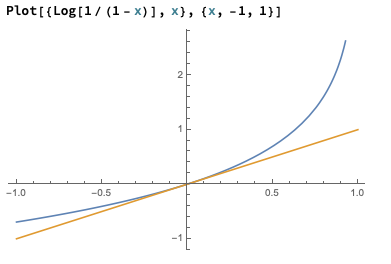
\includegraphics[width=0.5\linewidth]{fig/logbarrier.png}
%   \begin{minipage}{0.4\textwidth}
%     \centering
%     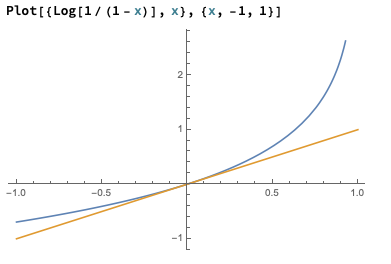
\includegraphics[width=0.9\textwidth]{fig/logbarrier.png} % first figure itself
%     \caption{Plot showing ${V(x) = -\log(1-x)}$ and then linear
%       approximation ${V(0) + V'(0) x}$.}
%   \end{minipage}\hfill
%   \begin{minipage}{0.4\textwidth}
%     \centering
%     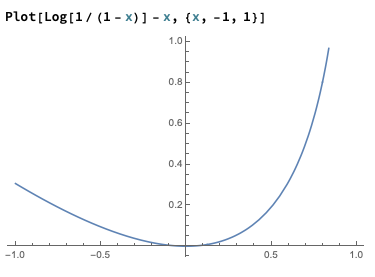
\includegraphics[width=0.9\textwidth]{fig/logdivergence.png}% second figure itself
%     \caption{Plot showing ${D(x) = V(x) - (V(0) + V'(0) x)}$.}
%   \end{minipage}
% \end{figure}


\begin{figure}[H]
  \centering
    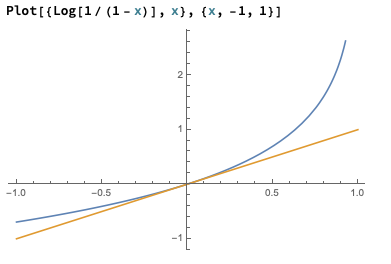
\includegraphics[width=0.6\textwidth]{fig/logbarrier.png} % first figure itself
    \caption{Plot showing ${V(x) = -\log(1-x)}$ and then linear
      approximation ${V(0) + V'(0) x}$.}
\end{figure}


\begin{figure}[H]
  \centering
    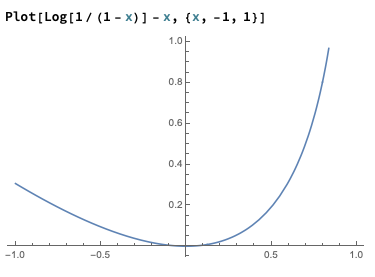
\includegraphics[width=0.6\textwidth]{fig/logdivergence.png}% second figure itself
    \caption{Plot showing ${D(x) = V(x) - (V(0) + V'(0) x)}$.}
\end{figure}

  
We let
\[
  \cc_+(e) = \cc(e) - \ff(e) \text{ and } \cc_-(e) = \cc(e) + \ff(e)
\]

So then  
\begin{align*}
  D_V( \ddelta )
  &=
  V(\ddelta+\ff)
  -
  (V(\ff)
  +
  \ip{\grad V(\ff), \ddelta})
  \\
  &=
  \sum_e
  -\log
  \left(\frac{\cc(e)-(\ddelta(e)+\ff(e))}
  {\cc(e)-\ff(e)} 
    \right)
   -
\frac{\ddelta(e)}
  {\cc(e)-\ff(e)} 
  \\
  &\quad\quad\,\,\,\,
  -\log
\left(
  \frac{\cc(e)+(\ddelta(e)+\ff(e))}
  {\cc(e)+\ff(e)} 
  \right)
   +
\frac{\ddelta(e)}
    {\cc(e)+\ff(e)}
  \\
  &=
    \sum_e
    D\left(\frac{\ddelta(e)}
    {\cc(e)-\ff(e)}
    \right)
    +
     D\left(-\frac{\ddelta(e)}
    {\cc(e)+\ff(e)}
    \right)
   \\
  &=
    \sum_e
    D\left(\frac{\ddelta(e)}{\cc_+(e)}\right)
    +
    D\left(-\frac{\ddelta(e)}{\cc_-(e)}\right)
\end{align*}

Note that we can express Problem~\eqref{eq:divflow} as
% \begin{equation}
%    \label{eq:divflow2}
% \begin{aligned}
%   \min
%   _{\ddelta \in \R^E} & \quad 
%      D_V( \ddelta )
%   \\
% \textrm{s.t. }  \BB\ddelta = \alpha' F^* \bb_{st}
% \end{aligned}
% \end{equation}
\begin{align}
   \label{eq:divflow2}
  \min_{\ddelta \in \R^E} & \quad 
      D_V( \ddelta )
  \\
  \textrm{s.t. }  \BB\ddelta = \alpha' F^* \bb_{st}
\tag*{The Update Problem, restated}
\end{align}

Note that  $D_V( \ddelta )$ is strictly convex of over the
feasible set, so the argmin is unique.

\subsection{Quadratically Smoothing Divergence and Local Agreement}

\[
  \sdiv_{\epsilon}(x) =
  \begin{cases}
    -\log(1-x) - x & \text{ if } \abs{x} \leq \epsilon \\
    D(\epsilon) + D'(\epsilon) (x - \epsilon) 
    +\frac{D''(\epsilon)}{2} (x - \epsilon)^2
    & \text{ if }  x > \epsilon \\
    D(-\epsilon) + D'(-\epsilon) (x + \epsilon) 
    +\frac{D''(-\epsilon)}{2} (x +\epsilon)^2
    & \text{ if }  x < -\epsilon \\
  \end{cases}
\]

For brevity, we define
\[
  \sdiv(x) =\sdiv_{0.1}(x) 
\]
\begin{lemma}
  \label{lem:sdivderivs}
  \noindent
  \begin{enumerate}
  \item $1/2 \leq \sdiv''(\xx) \leq 2$.
  \item For $x \geq 0$, we have $x/2 \leq \sdiv'(\xx) \leq 2x$
and $-2x \leq \sdiv'(-\xx) \leq -x/2$.
\item $x^2/4 \leq \sdiv(\xx) \leq x^2$.
  \end{enumerate}
\end{lemma}

What's happening here? We glue together $D(x)$ for small $x$ with its
quadratic approximation for $\abs{x} > \epsilon$.
For $x > \epsilon$, we ``glue in'' a Taylor series expansion based at $x =
\epsilon$.

\begin{figure}[H]
  \centering
    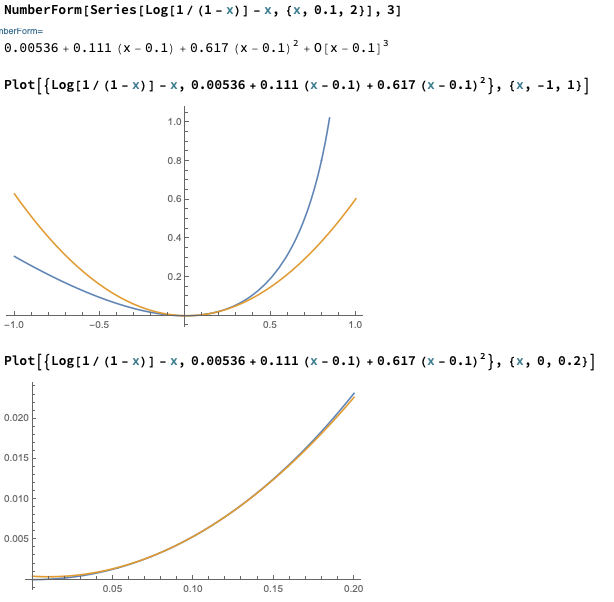
\includegraphics[width=\textwidth]{fig/quad-div-apx.png} % first figure itself
    \caption{Plot showing ${D(x) = -\log(1-x)}$ and the quadratic
      approximation based at $x = 0.1$.}
\end{figure}


We also define
  \begin{align*}
  \sdiv_V( \ddelta )
 &=
    \sum_e
     \sdiv\left(\frac{\ddelta(e)}{\cc_+(e)}\right)
    +
     \sdiv\left(-\frac{\ddelta(e)}{\cc_-(e)}\right)
  \end{align*}

We can now introduce the smoothed optimization problem
\begin{align}
   \label{eq:sdivflow}
  \min_{\ddelta \in \R^E} & \quad 
     \sdiv_V( \ddelta )
  \\
  \textrm{s.t. }  \BB\ddelta = \alpha' F^* \bb_{st}
\tag*{``The Smoothed Update Problem''}
\end{align}
Note that  $\sdiv_V( \ddelta )$ is strictly convex of over the
feasible set, so the argmin is unique.

\begin{pseudoclaim}
  We can compute the argmin $\ddelta^*$ of
  Problem~\eqref{eq:sdivflow}, the Smoothed Update Problem, using the Newton-Steps for
  $K$-stable Hessian convex functions that we saw in the previous chapter, in
  $\Otil(m)$ time.
\end{pseudoclaim}
\begin{proof}[Sketch of proof]
  Problem~\eqref{eq:sdivflow} fits the class of problems for which we
  showed in the previous chapter 
  that (appropriately scaled) Newton steps converge.
  This is true because the Hessian is always a $2$-spectral
  approximation of the Hessian at $\sdiv_V( \ddelta^* )$, as can be
  shown from Lemma~\ref{lem:sdivderivs}.
  Because the Hessian of $\sdiv_V( \ddelta )$ is diagonal, and the
  constraints are flow constraints, each
  Newton step boils down to solving a Laplacian linear system, which can
  be done to high accuracy $\Otil(m)$ time.
\end{proof}

\begin{remark}
  There are three things we need to modify to turn the pseudoclaim
  into a true claim, addressing the errors arising from both Laplacian
  solvers and Newton steps:
  \begin{enumerate}
  \item We need to rephrase the claim to so that we only claim
    $\ddelta^*$ has been computed to high accuracy, rather than exactly.
  \item We need to show that we can construct an initial guess to
    start off Newton's method $\ddelta_0$ for which the value
    $\sdiv_V( \ddelta_0 )$ is not too large. (This is easy).
  \item We need show that Newton steps converge despite using a
    Laplacian solver that doesn't give exact solutions, only high
    accuracy solutions. (Takes a bit of work, but is ultimately not
    too difficult).
  \end{enumerate}
Importantly, to ensure our overall interior point method still works,
  we also need to show that it converges,
even if we're using approximate solutions
everywhere. This also takes some work to show, again is not too difficult.
\end{remark}


\paragraph{Local Agreement Implies Same Optimum.}
\begin{lemma}
  \label{lem:argminsfromlocalagreement}
  Suppose $S \subseteq \R^n$ is a convex set, and let $f, g: S \to \R$ be convex
  functions.
  Let $\xx^* = \argmin_{\xx \in S} f(\xx)$.
  Suppose $f,g$ agree on a neighborhood of $\xx^*$ in $S$ (i.e. an
  open set containing $\xx^*$).
  Then $\xx^* = \argmin_{\xx \in S} g(\xx)$.
\end{lemma}
\begin{proof}[Proof Sketch]
  We sketch the proof in the case when both $f,g$ are differentiable: Observe
  that $\veczero = \grad f(\xx^*) = \grad g(\xx^*)$, and hence $g(\xx)$
  is also minimized at $\xx^*$.
\end{proof}

We define
\begin{equation}
  \label{eq:symrescap}
  \cchat(e) = \min(\cc_+(e) , \cc_-(e) ) 
\end{equation}
% and for a positive vector $\cc > 0$, we define
% \[
% \norm{\yy}_{\cc,\infty} = \norm{}
%   \]

\begin{lemma}
  Suppose $\ddelta^*$ is the argmin of
  Problem~\eqref{eq:sdivflow}, the Smoothed Update Problem, and
  $\norm{\cvec{\ddelta^*(e)/\cchat(e)}}_{\infty} < 0.1$.
  Then $\ddelta^*$ is the argmin of Problem~\eqref{eq:divflow2}.
\end{lemma}
\begin{proof}
  We observe that if   $\norm{\cvec{\ddelta^*(e)/\cchat(e)}}_{\infty}
  < 0.1$, then $\sdiv_V( \ddelta^*) = D_V( \ddelta^*)$, and,
  for all $\ttau \in \R^m$ with norm
  \[
    \norm{\cvec{\ttau(e)/\cchat(e)}}_{\infty} < 0.1 -
    \norm{\cvec{\ddelta^*(e)/\cchat(e)}}_{\infty}
  \]
  we have that
  $\sdiv_V( \ddelta^*+\ttau) = D_V( \ddelta^*+\ttau
  )$.
  Thus $\sdiv_V$ and $D_V$ agree on a neighborhood around
  $\ddelta^*$ and hence by
  Lemma~\ref{lem:argminsfromlocalagreement}, we have that
  $\ddelta^*$ is the argmin of Problem~\eqref{eq:divflow2}.
\end{proof}

\subsection{Step size for divergence update}

\begin{definition}[\emph{$s$-$t$ well-conditioned} graph]
   An undirected, capacitated multi-graph $G = (V,E,\cc)$ with source $s$
   and sink $t$ is 
   \emph{$s$-$t$ well-conditioned} if,
   letting $U$ denote the maximum edge capacity $U =
   \norm{\cc}_{\infty}$,
   we have at least $\frac{2}{3} m$ multi-edges of capacity $U$ going directly
   from $s$ to $t$.
 \end{definition}

 \begin{remark}
   It is straightforward to make a graph $s$-$t$ well-conditioned.
   We just add $2m$ new edges of capacity $U$ directly between $s$ and
   $t$.
   Given an exact maximum flow in the new graph, it is trivial to get
   one in the original graph: Just remove the flow on the new edges.
 \end{remark}
 
 \begin{definition}
   Given a \emph{directed} graph $G = (V,E,\cc)$, the
   \emph{symmetrization}
   of $G$ is the undirected $\Ghat = (V,\Ehat,\cchat)$ is the undirected graph given by
\[
\setof{a,b} \in \Ehat \text{ if } (a,b) \in E \text{ AND } (b,a) \in E    
\]
and
\[
  \cchat(\setof{a,b}) = \min(\cc(a,b),\cc(b,a))
  .
\]
\end{definition}
Note that when  $\Ghat_{\ff}$ is the symmetrization of the residual
   graph $G_{\ff}$ (which we defined in Chapter~\ref{cha:maxflow1}), then $\cchat$ matches
   exactly the definition of $\cchat$ in Equation~\eqref{eq:symrescap}.
\begin{lemma}
\label{lem:symres}
  Let $G$ be an undirected, capacitated multi-graph $G = (V,E,\cc)$
  which is $s$-$t$ well-conditioned.
   Let $\ff$ be the minimizer of Program~\eqref{eq:barrierflow}.
   Let $\Ghat_{\ff}$ be the \emph{symmetrization} of the residual
   graph $G_{\ff}$ (in the sense of Lecture~10).
   Then there exists a flow $\ddeltahat$ which satisfies $\BB \ddeltahat = \frac{1-\alpha}{5} F^*
   \bb_{st} $ and is feasible in
   $\Ghat_{\ff}$. Note that we can also state the feasibility in
   $\Ghat_{\ff}$ as
   \[
\norm{\cvec{\ddeltahat(e)/\cchat(e)}}_{\infty} \leq 1
     \]
\end{lemma}
\begin{proof}
  We recall since $\ff$ is the minimizer of
  Program~\eqref{eq:barrierflow}, there exists dual-optimal voltages
  $\xx$ such that
  \[
    \BB^{\trp} \xx = \grad V(\ff) =
    \cvec{\frac{1}
    {\cc(e)-\ff(e)}
    -
    \frac{1}
    {\cc(e)+\ff(e)}}
  \]
From Lecture~10, we know that there is flow $\ddeltabar$ that is feasible with
respect to the residual graph capacities of the graph $G_{\ff}$ such
that $\BB \ddeltabar = (1-\alpha)F^* \bb_{st}$.
Note when treating $\ddeltabar$ as an undirected
flow, feasibility in the residual graph means that $\ddeltabar(e) < \cc(e)-\ff(e)$
and $-\ddeltabar(e) < \cc(e)+\ff(e)$.
Thus,
\[
  (1-\alpha)F^* \bb_{st}^{\trp}
  \xx
  =
  \ddeltabar 
  \BB^{\trp} \xx
  =
  \sum_e
  \frac{\ddeltabar}
    {\cc(e)-\ff(e)}
    -
    \frac{\ddeltabar}
    {\cc(e)+\ff(e)}
    \leq
    m
  \]
  Now, because the graph is $s$-$t$ well-conditioned,
  there are at $\frac{2}{3} m $ edges directly from $s$ to $t$ with capacity $U$
  and each of these $e$
 satisfy by the Lagrangian gradient optimality condition~\eqref{eq:barrierlagrangegrad}
 \[
   \bb_{st}^{\trp}
  \xx
   =
  \frac{1}
    {U-\ff(e)}
    -
    \frac{1}
    {U+\ff(e)}
  \]
Note that $\frac{2}{3} mU \leq F^* \leq mU$ because the graph is $s$-$t$
well-conditioned.
To complete the analysis, we consider three cases.

\emph{Case 1: $\abs{\ff(e)} \leq \frac{2}{3} U$.}
Then the capacity on each of these edges in the symmetrized residual
graph $\Ghat_{\ff}$ is at least $U/3$.
As there are $\frac{2}{3} m $ of them,
we get that there is a feasible flow in $\Ghat_{\ff}$ of value at least
$\frac{2}{9} mU\geq \frac{1}{10} F^*$. 

\emph{Case 2: $\ff(e) < -\frac{2}{3} U$.}
By the gradient condition, we have the same flow on all of the $\frac{2}{3} m$
$s$-$t$ edges, adding  up to at least $\frac{2}{3} mU$ going from $t$ to $s$.
This means that we must have at least $\frac{2}{3} mU$ flow going from
$s$ to $t$ via the remaining edges. But, their combined capacity is at
most $\frac{1}{3} mU$, so that cannot happen. Thus we can rule out
this case entirely.

\emph{Case 3: $\ff(e) > \frac{2}{3} U$.}
Then 
\[
  \frac{m}{(1-\alpha)F^* }
  \geq
     \bb_{st}^{\trp}
     \xx
 \geq
  \frac{1}
    {U-\ff(e)}
    -
    \frac{1}
    {U+\ff(e)}
 \geq
   \frac{4/5}
    {U-\ff(e)}
  \]
So
\[
  U-\ff(e) \geq \frac{4}{5}  \frac{(1-\alpha)F^* }{m}
  \geq \frac{1}{2}
(1-\alpha) U
\]
In this case, the capacity on each of the $\frac{2}{3} m$ 
$s$-$t$ edges with capacity $U$ in $G$ will
have capacity $(1-\alpha) U/2$ in $\Ghat_{\ff}$.
This guarantees that there is feasible flow in $\Ghat_{\ff}$ of value
at least $\frac{1}{3} (1-\alpha) mU \geq \frac{1}{3} (1-\alpha) F^*$.
\end{proof}
\begin{lemma}
  Let $0 < \alpha' \leq \frac{1-\alpha}{150\sqrt{m}}$.
  Then the minimizer $\ddelta^*$ of Problem~\eqref{eq:sdivflow}
  satisfies $\norm{\cvec{\ddelta^*(e)/\cchat(e)}}_{\infty} < 0.1$.
\end{lemma}
\begin{proof}
  By Lemma~\ref{lem:symres}, there exists a flow $\ddeltahat$ which satisfies $\BB \ddeltahat = \frac{1-\alpha}{5}  F^*
   \bb_{st} $ and ${\norm{\cvec{\ddeltahat(e)/\cchat(e)}}_{\infty} \leq
   1}$.
 Hence for any
 $0 < \alpha' \leq \frac{1-\alpha}{150\sqrt{m}}$,
 the flow 
 $\ddeltatil = \alpha' \frac{5}{1-\alpha}\ddeltahat$
 satisfies
$\BB \ddeltatil = \alpha' F^*\bb_{st}$
and
$\norm{\cvec{\ddeltatil(e)/\cchat(e)}}_{\infty}
\leq
\frac{1}{30\sqrt{m}} $.
   This means that
\begin{align*}
     \sdiv_V( \ddeltatil )
     &=
    \sum_e
     \sdiv\left(\frac{\ddeltatil(e)}{\cc_+(e)}\right)
    +
    \sdiv\left(-\frac{\ddeltatil(e)}{\cc_-(e)}\right)
  \\
  &\leq
    \sum_e
     4\left(\frac{\ddeltatil(e)}{\cc_+(e)}\right)^2
    +
    4\left(-\frac{\ddeltatil(e)}{\cc_-(e)}\right)^2
  \\
  &
  \leq
    \sum_e
    8\left(\frac{\ddeltatil(e)}{\cchat
        (e)}\right)^2
 \\
     &\leq 8/900 < 1/100
.
\end{align*}

This then means that the minimizer $\ddelta^*$ of
Problem~\eqref{eq:sdivflow} also satisfies
$\sdiv_V( \ddeltatil ) < 1/100$.

\begin{align*}
  \norm{\cvec{\ddelta^*/\cchat(e)}}_{\infty}^2
&\leq 
      \sum_e
     \left(\frac{\ddelta^*(e)}{\cc_+(e)}\right)^2
    +
    \left(-\frac{\ddelta^*(e)}{\cc_-(e)}\right)^2
\\                                      
&\leq 
    \sum_e
     \sdiv\left(\frac{\ddelta^*(e)}{\cc_+(e)}\right)
    +
    \sdiv\left(-\frac{\ddelta^*(e)}{\cc_-(e)}\right)
\tag*{By Lemma~\ref{lem:sdivderivs}.}
\\
  &=
\sdiv_V( \ddeltatil ) 
<
1/100
.
\end{align*}
Hence $\norm{\cvec{\ddelta^*/\cchat(e)}}_{\infty} < 0.1$.
\end{proof}


% \todo{writing plan}
%  \begin{itemize}
%  \item well-cond def
%  \item symmetrized res graph
%  \item  state existence of a big, feasible step in sym-res graph (inf norm)
%    (asym -> sym)
%  \item use of that to say that smoothed divergence opt is within $\infty$
%    ball for 
%  \item prove existence proof of the step
%  \end{itemize}
 
% \begin{definition}
% Given a feasible flow $\ff$ in $G = (V,E,\cc)$
% \end{definition}

% \begin{lemma}
%    Suppose the original graph is $G = (V,E,\cc)$ is \emph{$s$-$t$
%      well-conditioned},
%    and suppose $\ff$ is the 
% \end{lemma}

% Suppose the original graph is $G = (V,E,\cc)$ is \emph{preconditioned}


% \subsection{old step size writing}

% We define a strict barrier feasbility condition:
% \begin{align}
%   \label{eq:strictbarrierfeasibility}
%   \BB\ff= \alpha F^* \bb_{st}
%   \text{ and }
%   -\cc < \ff < \cc
%   \\
%   \tag*{"Strict barrier feasibility"}
% \end{align}
 
% \begin{lemma}
%   Suppose $\ff$ is a flow  satisfying the strict barrier
%   feasibility conditions.
%   Note that 
%   Consider 
%   There exists a flow $\ddelta_{\infty}$ s.t.
% \end{lemma}

% oops

% \begin{itemize}
% \item the problem is that if we SUBSTANTIALLY use a forward edge
% \item then we still need to make sure it doesn't exceed the backward
%   edge capacity :(
% \end{itemize}

% \todo{you can leave comments like this}


%%% Local Variables:
%%% mode: latex
%%% TeX-master: "agao21_script"
%%% End:
